\chapter{La méthode Tomatis}

\section{Historique :}

Alfred Tomatis est né le 1er janvier 1920 et décédé le 25 décembre
2001. Il était docteur en médecine, spécialiste en oto-rhino-laryngologie,
connu mondialement pour ses travaux sur l'audition et la phonation.
Spécialisé particulièrement en neurophysiologie auditive, il a créé
une nouvelle discipline, l'audio-psycho-phonologie. Il a consacré
une grande partie de son activité professionnelle à étudier le relation
existante entre l'oreille et la voix, et par extension entre l'écoute
et la communication. Il s'agit de plus de cinquante ans de recherches
sur les fonctions de l'oreille. Ses découvertes furent établies au
laboratoire de physiologie de la Sorbonne et donnèrent lieu à des
communications à l'Académie des Sciences et à L'Académie de Médecine
de Paris en 1957 et 1960. Son oeuvre représente plusieurs dizaines
de publications ainsi que treize ouvrages. (Cf.bibliographie)

\section{Définition : La Méthode Tomatis}

La Méthode Tomatis, créée par le sus-nommé, est une pédagogie et une
thérapie de l'écoute. Son outil est un appareil électronique appelé
Oreille Electronique. (cf.chap.3.4.) Celui-ci est un appareil d'éducation
et/ou de rééducation. On parle d 'effet Tomatis qui permettrait au
cerveau d'améliorer naturellement \emph{l'interprétation du message
sensoriel.}

\paragraph{L'audio-psycho-phonologie, créée par Tomatis, aborde l'écoute comme
clé de décodage pour comprendre l'homme.}

Tomatis était avant tout un clinicien à l'écoute de ses patients avec,
pour motivation première, l'application clinique de ses recherches.
Guidé par son intuition avec la faculté de remise en question des
théories appliquées ainsi que celle de créer des liens entres les
disciplines, Tomatis a pu élaborer un nouveau type de thérapie, dénommée
l'audio-psycho-phonologie. Elle regroupe trois disciplines, successivement,
l'audio (l'oreille) la psychologie et la phonologie( voix). La voix
dépend de l'oreille et sont, tous les deux, des outils de la communication
(psychologie). Cette façon de regrouper les disciplines se retrouve
aujourd'hui de plus en plus, que ce soit, par exemple en psycho-neuro-immunologie
(PNI)devenue actuellement discipline médicale de pointe.\footnote{La PNI étudie l'impact des événements psychiques sur le système immunitaire.
Elle repose sur la mise en évidence d'interrelations entre le système
nerveux central, le système neuroendocrinien et le système immunitaire.
C'est une approche interdisciplinaire incorporant des données de la
psychologie, de la neuroscience, de la neurologie, dont l'endocrinologie
et l'immunologie.( entre autres) Source : Wikipédia, février 17.}Tomatis accorde à l'oreille une place extrêmement importante. En soignant
des chanteurs à la voix déficiente, il a eu l'idée de leur tester
leur audition et a ainsi détecté des correspondances avec leurs difficultés
vocales.

De là, il énonce les lois qui constituent ``l'effet Tomatis'' : 
\begin{itemize}
\item La voix ne contient que ce que l'oreille entend.
\item Si l'on modifie l'audition, la voix est immédiatement et inconsciemment
modifiée.
\item Il est possible de transformer la phonation par une stimulation auditive
entretenue pendant un certain temps ( loi de rémanence).
\end{itemize}
Cette méthode répond ainsi à des objectifs variés: éducatifs : apprentissages
des langues, de la musique ; rééducatifs : troubles psychologiques,
moteurs, troubles du langage ; et psychothérapeutiques : angoisse,
dépression. 

Elle agit simultanément sur trois fonctions essentielles de l'oreille
: l'audition, l'équilibre et la dynamisation.
\begin{itemize}
\item Audition : lorsque l'on s'entend , on peut mieux se structurer.
\item Réharmonisation : équilibre et coordination : le SNC (système nerveux
central) est touché lors de l'écoute de musique par l'intermédiaire
du vestibule. Il y a une action sur les troubles psychomoteurs, les
réponses motrices deviennent plus fluides. Les dysfonctionnements
correspondent à un état de non-équilibre neurophysiologiques plus
ou moins prononçés. Le travail sous Oreille Electronique va tendre
à faire revenir le sujet à un état d'équilibre : ainsi les progrès
observés se maintiennent et ne sont donc pas dûs à un conditionnement.
Le processus d'évolution a été rétabli dans sa normalité.
\item Stimulation : dynamiser le cerveau par des fréquences spécifiques
et par là-même le corps tout entier. Le son est nécessaire pour notre
épanouissement personnel. L'oreille a besoin d'être stimulée pour
énergiser le cerveau et le corps. En privilégiant les musiques avec
de grandes gerbes harmoniques( élevées, aigues) on induit la stimulation
de la formation réticulée. En captant des milliers d'informations
à chaque instant, l'oreille recharge le cerveau et lui permet d'être
à l'écoute de soi et des autres. Pour qu'un cerveau ``fonctionne'',
il lui faut trois milliards de stimulations par seconde.
\end{itemize}
A ce rôle prédominant de l'oreille se greffe une grande diversité
de champs d'application. Celle-ci est due à une conception intégrative
de l'homme, puisqu'elle met en interaction toutes ses dimensions corporelles
et psychologiques ; cette forme de thérapie prend en compte le corps,
les émotions et les cognitions. On pourrait la considérer comme holistique.
La PNL, l'Hypnose eriksonnienne ou l'EMDR( Eye Movement Desensitization
and Reprocessing) en sont des autres exemples. 

Cette nouvelle forme de thérapie et de pédagogie est basée sur une
théorie différente de la physiologie auditive classique et a été élaborée
de manière clinique pendant de nombreuses années . Elle est le fruit
d'expérience et de preuves par résultats. Elle a suscité beaucoup
de réactions et de critiques en milieu médical. Nous reviendrons plus
en détails sur ce sujet dans le chapitre suivant. De manière générale,
on conteste sa nouvelle compréhension de l'oreille.

Ainsi il s'avère nécessaire de décrire brièvement l'anatomie de l'oreille
avec le vocabulaire qui s'y associe et qui nous sera utile.

\section{L'oreille : description : }

\subsection{L'anatomie de l'oreille :}
\begin{figure}
	\centering
	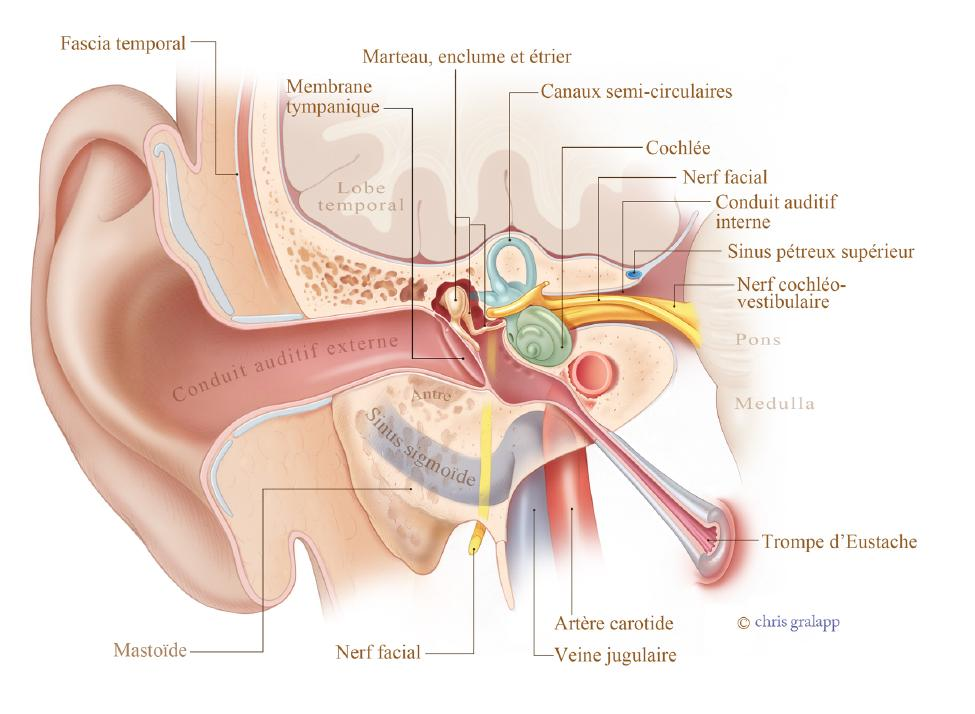
\includegraphics[width=0.7\linewidth]{images/20160624Berufsfeldgruppen.jpg}
	\caption[Titre pour toc]{Titre long pour la page}
	\label{fig:-20160624berufsfeldgruppen}
\end{figure}


(canal auditif). Les ondes sonores entrent dans le méat et percutent
une membrane de 60 mm2, appelée tympan, et la font vibrer. Cette membrane
sépare l'oreille externe de l'oreille moyenne. Selon Tomatis, elle
joue un rôle de filtre des graves et d'amplificateur des aigus.\footnote{Biologie humaine, principes d'anatomie et de physiologie, Elaine N.Marieb,
éd.Pearson Education, 8ème édition, chap. 8, pp.319-321}

L'oreille moyenne : se trouve dans l'os temporal constituée de petites
cavités dont une, centrale, qui est la caisse du tympan. Sa limite
médiale est une paroi osseuse percée de deux orifices , la fenêtre
du vestibule et la fenêtre de la cochlée. La trompe auditive ou d'Eustache
est un conduit oblique qui relie l'oreille moyenne à la gorge et sert
à équilibrer la pression de l'air entre l'oreille moyenne et l'extérieur.
Les trois osselets de l'ouïe sont : le marteau, l'enclume et l'étrier
( les plus petits os du corps). Ils transmettent les vibrations du
tympan aux liquides de l'oreille interne. Le marteau et l'étrier sontse
trouve dans l'os temporal constituée de petites cavités dont une,
centrale, qui est la caisse du tympan. Les trois osselets de l'ouïe
sont : le marteau, l'enclume et l'étrier ( les plus petits os du corps);
le marteau et l'étrier sont commandés chacun par un muscle. D'après
Tomatis, son rôle est double : protéger l'oreille interne des sons
trop forts et celui de cibler les sons à écouter.


L'oreille interne : est l' organe de l\textquoteright audition. Il
est constitué d'une coque osseuse d'une très grande densité( la plus
importante du corps), contenant un corps membraneux qui en épouse
la forme. L'oreille interne est une enfilade de cavités osseuses portant
le nom de labyrinthe osseux. Il comprend trois subdivisions : la cochlée,
le vestibule du labyrinthe et les canaux semi-circulaires. Le labyrinthe
osseux est rempli de périlymphe, un liquide. Et dans ce périlymphe
flotte le le labyrinthe membraneux qui contient lui-même un liquide
plus épais appelé endolymphe. Ils jouent leur rôle dans l'équilibre
statique et dynamique.Le vestibule et les canaux semi-circulaires
sont les organes de l\textquoteright équilibration , la cochlée ou
limaçon est l'organe de l'audition. 


\subsection{La physiologie de l'oreille : }

Le chemin du son dans l'oreille jusqu'au cerveau : 

Chaque son parvenant à l'oreille entre dans le pavillon et se propage
dans le conduit auditif. Les vibrations de l'onde sonore mettent en
mouvement le tympan lié aux trois petits os (marteau, enclume, étrier).
La transformation (et l\textquoteright amplification) des vibrations
aériennes en vibrations solidiennes se fait par l\textquoteright intermédiaire
des osselets : les vibrations du tympan entraînent successivement
celles du bloc marteau-enclume puis celle de l\textquoteright étrier,
qui les transmet à l\textquoteright oreille interne via la fenêtre
ovale.

Le rapport de levier effectif entre le marteau et l\textquoteright enclume
(de l\textquoteright ordre de 20), d\textquoteright une part, et le
rapport de surfaces entre le tympan (60mm2) et la platine de l\textquoteright étrier
(30 mm2) d\textquoteright autre part font du système tympano-ossiculaire
un véritable amplificateur permettant à l\textquoteright énergie sonore
d\textquoteright être transmise presque intégralement à l\textquoteright oreille
interne.

A partir de 80 dB, un réflexe protecteur (stapédien) est mis en place
afin de réduire la transmission des pressions vers l\textquoteright oreille
interne, par l\textquoteright intermédiaire des osselets et des muscles
qui rattachent le marteau et l\textquoteright étrier aux parois de
la caisse du tympan. Il s'agit ainsi d' un procédé mécanique qui amplifient
les vibrations atteignant la cochlée. 
\begin{quotation}
La cochlée à son tour ``va transformer ces vibrations en impulsions
nerveuses véhiculées par le nerf auditif.'' (...)Les cellules ciliées
tapies dans la membrane cochléaire ``transforment ces vibrations
en messages électriques, circulant dans le nerf auditif. (...) Et
ces informations vont ``se diriger vers le cortex cérébral, via plusieurs
relais.(...) ``Comme certaines fibres issues de chaque oreille croisent
la ligne médiane, chaque aire auditive reçoit des signaux des deux
oreilles.'' De plus, ``tout au long du trajet, le message subit
des transformations dues aux caractéristiques de l'activité des neurones.''
Retenons que `` les cellules ciliées proches de l'étrier sont activées
par les sons aigus, et celles situées au sommet de la cochlée le sont
par les sons de basse fréquence''.(...) `` Une scène auditive est
mêlée d'un ensemble d'ondes acoustiques et son analyse se ferait non
seulement tout au long du système auditif avec des indices comme la
fréquence et l'intensité mais aussi au-delà, pour utiliser les informations
liées aux autres sens ou au contexte.'' \footnote{\cite{AuteurInconnu2011}, pp.~15--16.}
\end{quotation}

\section{Critiques et interrogations :}

Tomatis s'oppose sur plusieurs points aux théories classiques de la
physiologie auditive : 
\begin{itemize}
\item l'oreille moyenne et son rôle de transmetteur 
\item l'analyse fréquentielle au niveau de la cochlée
\end{itemize}
Son originalité réside dans sa conception de la transmission du son
au niveau de l'oreille interne. 

Il propose une nouvelle compréhension de l'oreille, celle-ci étant,
à son regard, un organe actif dans le sens suivant :
\begin{itemize}
\item L'oreille moyenne, grâce aux muscles de l'étrier et du marteau, fait
un travail de visée en ciblant les sons à écouter : le tympan se tend
pour se mettre en résonance avec les sons à percevoir.
\item Il fait aussi un autre travail qui est celui de sélectionner des sons
pour se protéger : la tension tympanique se détend pour amortir l'intensité
sonore qui inonde l'oreille interne. 
\end{itemize}
\begin{description}
\item [{Selon}] la théorie de Georg Békésy, qui obtint le prix Nobel de
physiologie en 1961 et qui reste encore la référence classique, l'oreille
ne sert qu'à transmettre les sons de manière passive comme peut le
faire un micro. Le rôle des osselets se limite à la transmission du
son. Comme déjà décrit plus haut, les sons font vibrer le tympan qui,
étant attaché au marteau, répercute ces ondes acoustiques en mouvements
mécaniques via les osselets. L'étrier transmet ensuite ces mouvements
à l'oreille interne en jouant comme un piston au niveau de la fenêtre
ovale. L'information acoustique est alors transmise sous forme d'ondes
liquidiennes ou encore de tourbillons. Les tourbillons sont analysés(
amplitude et vitesse) en termes de fréquences et de volume par les
cellules ciliées qui tapissent l'oreille interne. 
\item [{Selon}] Tomatis, cette théorie a de nombreuses incohérences. L'une
d'entr' elles serait que cette démonstration ne marche qu'avec un
son pur \footnote{un son pur est constitué d'une unique fréquence ou onde}.
Or, les sons purs n'existent pas dans la nature, car ils sont, au
contraire, complexes et formés d'une multitude de fréquences et d'intensités
variées. Et cette complexité ne peut pas être transmise sans perte
et instantanément par des mouvements mécaniques et retransformée en
tourbillons. De plus, il y a un espace entre l'enclume et l'étrier,
microscopique à l'oeil nu mais énorme sur un plan comparatif, c'est
un hiatus considérable à l'échelle atomique puisqu'il est de l'ordre
d'un millimètre. Ce phénomène reste inexpliquable sur le plan de la
physique pure.
\end{description}
\footnote{Conférence au IIème Congrès International d'Audio-Psycho-Phonologie
Paris 1972 \emph{: Nouvelles théories sur la physiologie auditive}} : il est de l'ordre de s'interroger s'il est possible que la transmission
puisse se faire dans ces conditions. On peut imaginer que le son passe
partout, par les ligaments de jonction des osselets ou les espaces
inter-ossiculaires mais

ce n'était pas scientifiquement prouvable lors d'une de ses conférences
en 1972. Peut-être l'est-il à l'heure actuelle, mais nous n'en avons
pas trouvé trace. 

Nous allons aborder la conduction osseuse qui pourrait nous aider
dans cette compréhension.
\begin{description}
\item [{La}] conduction osseuse : lorsque l'on fait l'expérience de se
boucher les oreilles et de parler normalement, on se rend compte que
notre voix se propage principalement par les os de la tête. Comment
expliquer que l'on perçoive parfaitement bien les sons par conduction
osseuse en mettant un vibrateur conducteur de son sur la boîte crânienne
? et ce, même si l'oreille moyenne est abîmée ( tympan percé, osselets
non fonctionnels) . Selon une dernière recherche, effectivement, le
son stimule l'oreille de deux manières : par voie aérienne en transitant
par les trois parties de l'oreille et par voie osseuse en stimulant
directement l'oreille interne par vibrations des structures osseuses
qui l'entourent. Ce site : oreillemudry.ch a été mis à jour le 28.07.2016.
Il relève l'importance de la voie osseuse mais ne signale aucun nouvel
élément dans la transmission fréquentielle que celle dite classique,
évoquée plus haut. 
\item [{Schéma:}] Physiologie de l\textquoteright audition 
\item [{D'après}] Tomatis, les sons arrivent bien par le canal auditif
jusqu'au tympan. L'onde acoustique excite la membrane tympanique et
par voie de conséquence, l'os de la caisse du tympan. A l'instar d'une
peau de tambour qui fait chanter le bois auquel elle est attachée,
c'est toute la boîte crânienne qui inondée de sons et en particulier
l'oreille interne. Celle-ci, de par sa grande densité, capte les sons
et résonne comme du cristal. (\marginpar{ La transmission du son par l'os est de 5000 m/s.}
Les fréquences qui forment les sons vont ainsi exciter les cellules
ciliées qui tapissent la cochlée, tel un piano enroulé. 
\item [{Avec}] sa théorie, l'analyse multifréquentielle ne se pose plus
: chaque fréquence se dirige instantanément et naturellement\emph{
}vers la cellule ciliée qui lui correspond. C'est grâce à la forme
particulière\emph{ }du limaçon qu'il y a un tri fréquentiel instantané.
Le son identique fréquentiellement s'installe toujours au même endroit,
sur une ligne isofréquentielle, qui est une tranche perpendiculaire
à l'axe.
\end{description}
Et le phénomène des tourbillons n'a donc pas pour fonction de transmettre
les sons mais interviennent pour déclencher les mécanismes d'adaptation
aux bruits. 
\begin{description}
\item [{Comment}] cela se passse-t-il ? Lorsque l'intensité des sons augmente,
l'excitation des cellules ciliées provoque des perturbations liquidiennes
dans l'oreille interne, c.à.dire des tourbillons. Ceux-ci se propagent
et sont amortis par l'étrier. Si les sons atteignent une intensité
dangereuse pour les cellules ciliées, l'étrier réagit fortement et
entraîne une réaction du marteau qui modifie la tension du tympan.
A son tour, le tympan, relâché, amortit le volume sonore transmis
à l'oreille interne, comme la paupière qui se ferme quand la lumière
est trop intense.
\end{description}

\subparagraph*{``Le tympan se met dans un certain état de tension pour jouer le
rôle d\textquoteright un diapason qui fait vibrer toute la boîte cranienne
par l'intermédiaire du sulcus tympani. \emph{C'est toute la boîte
crânienne qui vibre et qui transmet le son à la vésicule labyrinthique
et non à la chaîne ossiculaire que l'on a l'habitude de considérer
comme le véhicule du son. }La chaîne ossiculaire est un ensemble qui
joue le rôle d'adaptateur, de régulateur et non de transmetteur. La
conduction du son par l\textquoteright air puis par l'os doit donc
être étudiée d\textquoteright une façon complémentaire afin que l'on
puisse déterminer par la suite la posture d'écoute du sujet.''\protect\footnote{key 14, Entretien réalisé par B.Auriol avec Tomatis, Anvers 1973}}

Nous avons tenté  une étude comparative des
recherches actuelles au sujet de la physiologie auditive mais à notre connaissance, nous n'avons rien de nouveau à ce sujet.

Christine Petit note et relève par ces recherches le rôle important
et indéniable de la cochlée sur notre audition et spécifie qu'encore
à l'heure actuelle, il reste très mystérieux. \nomenclature{cochlée}{Anatomie : organe de l'audition,appareil sensoriel, en forme de spirale, la cochlée, incluse dans l'os du rocher, forme le limaçon membraneux ,se situe dans l'oreille interne et permet de déceler des sons extrêmement faibles, de discréminer des fréquences et de masquer des sons faibles par des sons forts. }
''C'est une sorte de minuscule appareil électroacoustique capable
de discréminer des sons extrêmement faibles, capable de \emph{masquer
les sons faibles par des sons forts}, pouvant \emph{distordre les
sons,} et en conséquent, \emph{capable d'élaborer un traitement extrêmement
sophistiqué des sons}.''

\footnote{ Christine Petit, titulaire de la chaire Génétique et physiologie
cellulaire au Collège de France, entretien en novembre 2012, réalisé
par Laurent Salters et Vincent Gaullier, Look at science : le système
sensoriel auditif confirme lors d'un entretien réalisé en 2012 le
rôle indéniable de la cochlée. key-13}
\begin{description}
\item [{Observation}] et critiques sur l'application et l'utilisation de
la méthode Tomatis : 
\item [{C'est}] une méthode controversée car il manque des études médicales
de grande envergure sur le sujet, susceptibles d'une évaluation statistique
sûre. Selon Pierre Lane, journaliste de l'émission Envoyé spécial
\footnote{Emission télévisée ``Envoyé spécial''16.5.1991}, Tomatis
a inventé une méthode qui est très critiquée mais qui a donné des
résultats. Elle ouvre l'oreille par des procédés mécaniques pour atteindre
des domaines spécialisés , que ce soit en médecine, en psychologie,
en ostéopathie, etc. Pierre Lane précise qu'il s'agit d'un outil proposé
en complément de leur pratique à de nombreux spécialistes. 
\item [{Au}] fil des années, de nombreuses études scientifques et cliniques
ont été faites. Il est possible d'en trouver le contenu sur le site
internet officiel Tomatis : Tomatis Research and Publication des plus
anciens aux plus récents en 2016.\footnote{www.tomatisassociation.org}
Nous pouvons citer les travaux des Docteur Du Plessis sur l'effet
Tomatis sur l'anxiété en milieu scolaire et universitaire,\footnote{Troubles psychologiques : Etude du Plessis (Université de Potchefstroon
- Afrique du Sud)avec un comparatif Pre / Post niveau d\textquoteright anxiété.
Du Plessis a étudié le cas de 29 étudiants sujets à l\textquoteright anxiété.
10 étudiants ont suivi des séances d\textquoteright écoute Tomatis\textregistered ,
9 ont suivi une psychothérapie classique et 10 ont été choisis pour
former le groupe contrôle. Le groupe Tomatis\textregistered{} a montré
une réduction significative de l\textquoteright anxiété, tandis que
les resultats sont mitigés pour ceux qui ont suivi une psychothérapie
et inexistants pour le groupe contrôle.

Une seconde étude De Plessis a démontré qu\textquoteright après 14,3
mois le niveau d\textquoteright anxiété avait continué à baisser fortement
pour le groupe Tomatis\textregistered{} alors qu\textquoteright aucun
changement n\textquoteright apparaissait pour le groupe contrôle.} \footnote{Du Plessis W.F. and Van Jaarsveld, P.E.(1988), \emph{Audio-psycho-phonology
: A comparative outcome study on anxious primary school pupils, }S\emph{.}Afr.
Tydskr.Sielk.1988,18(4)144-151;

Du Plessis,W.F., Burger,S.(2001)(..) \emph{A pilot study involving
the Tomatis method.}Sud Africa J.Psychol. et plus récemment encore
(2004) \emph{The Impact of a Combined Tomatis and Psycho-Educational
Program on Weight Preoccupied, Female south African Students, }International
Journal of Tomatis Method Research,1(1)54-65} les travaux de Jan Gerritsen, PhD (2009) \footnote{\emph{A Review of Research done on Tomatis Auditory Stimulation}},
les études du dr.P.E.Van Jaarsveld, psychologue à l'Université de
Potchefstroom en Afrique du Sud sur l'action de l'audio-psycho-phonologie
sur le bégaiement \footnote{\emph{The Effect of Audio-Psycho-Phonology on Stuttering}}.
\item [{Plus}] récemment nous citerons encore en dernier lieu la parution
de la dernière recherche menée en collaboration avec le CNRS. Cette
recherche a été publiée dans la revue scientifique \char`\"{}Journal
of Affective Disorders\char`\"{}. Elle a donc fait l'objet d'une validation
par un comité de lecture scientifique. Elle démontre qu'il existe
un lien important et certain entre la difficulté à percevoir certains
sons et l'existence de troubles émotionnels. L'intérêt de stimuler
le cerveau en lui permettant de capter plus facilement ces sons est
donc dès lors évident. Il s'agit d'une étude pilote du Dr.Carlos Escera
de l'Université de Barcelone en 2014 \footnote{\begin{description}
\item [{\emph{http://tomatisassociation.org/scientific-validation-of-the-tomatis-effect-eeg-recordings-of-sound-from-brainstem-to-cerebral-cortex-encoding-university-of-barcelona-2014/}}]~
\end{description}
}sur l'effet d'une technique particulière employée avec l'Oreille Electronique
-la bascule électronique \footnote{( qui permet de créer une alternance entre deux conditions perceptives
du même message sonore -passage soudain et imprévu de fréquences graves
à des fréquences aigues) . }
\item [{Nous}]~
\end{description}
\emph{}\footnote{\emph{``Les seuils auditifis des sons purs sont diminués chez les
personnes déprimées avec des troubles de stress post-traumatique.''}
\begin{description}
\item [{\emph{\char`\"{}Pure-tone}}] \emph{auditory thresholds are decreased
in depressed people with post-traumatic stress disorder\char`\"{}
Journal of Affective disorders.} Recherche du CNRS en collaboration
avec Tomatis Developpement S.A.
\end{description}
Auteurs : Stéphanie Aubert-Khalfa; Emmanuelle Reynaud; Myriam El Khoury;
Olivier Blin - INCM, UMR CNRS 6193, Jean-Pierre Granier - TOMATIS
DEVELOPPEMENT S.A. Eva-Maria Grosse; Jean-Claude Samuelian - Pôle
Psychiatrie Centre, La Conception Hospital }

Il y a lieu d'observer et de remarquer que certaines de ces études
ont été menées en collaboration avec la société Tomatis actuelle,
ce qui enlève quelque peu l'intégrité de la recherche.
\begin{quotation}
Selon le Dr.med.Inge Flehming\footnote{Dr.med.Inge Flehming, neurologue, neuropédiatre, texte publié en allemand
en 1996,\emph{``Grundsatz-Gutachten zur Behandlungsmethode nach Prof.Tomatis''http://www.analytische-hoertherapie.de/uploads/tx\_templavoila/Grundsatzgutachten\_zur\_Behandlungsmethode\_nach\_Prof.\_Tomatis.pdf}}''il est compréhensible que les médecins ORL n'en soient pas convaincus
par le fait que les objectifs thérapeutiques sont différents. L'ORL
cherche à améliorer l'audition tandis que le neurologue ou le neuropédiatre
ne s'en préoccupe pas, mais cherche à comprendre les raisons pour
lesquelles certains sujets ont des difficultés à appréhender ce qu'ils
entendent, c'est-à-dire à traiter correctement l'information au niveau
du cerveau.''
\end{quotation}
\begin{quote}
\footnote{``Or le traitement central correct d'un stimulus relayé au cerveau
par les voies sensorielles présuppose l'acquisition d'une synergie
parfaite entre les systèmes sensoriels au niveau de l'organe central
(le cerveau), un processus nommé \char`\"{}intégration sensorielle\char`\"{}.
Dans ce contexte, Tomatis distingue entre \char`\"{}l'audition\char`\"{},
prise comme l'expression de la réalisation acoustique de l'impulsion
auditive dans le cerveau, et \char`\"{}l'écoute\char`\"{}, prise comme
un processus \char`\"{}d'écoute consciente\char`\"{}, impliquant l'attention
immédiate et la conscience subjective de l'individu. En présence d'une
stimulation adéquate, toutes les voies sensorielles du corps sont
en mesure de réaliser l'intégration sensorielle, prise comme synergie
des systèmes sensoriels, et leur interconnexion au niveau du cerveau.
L'oreille joue néanmoins un rôle tout à fait particulier dans ce processus.
En effet, le labyrinthe osseux de l'oreille interne réunit deux systèmes
sensoriels diamétralement opposés, mais néanmoins fondamentaux, l'un
et l'autre, dans un espace très réduit. Le système auditif est le
premier système sensoriel achevé sur le plan anatomique dans l'évolution
prénatale de l'enfant. Cela veut dire que dès une phase précoce de
la grossesse, l'audition est entièrement opérationnelle, et mise à
contribution. De nos jours, nous savons que la formation de synapses
entre les neurones du cerveau, c'est-à-dire le câblage et l'interconnexion
des milliards de neurones présents dans le cerveau, obéit à un processus
activement contrôlé, où des dendrites \char`\"{}chercheurs\char`\"{}
et des dendrites \char`\"{}récepteurs\char`\"{}, guidés en-cela par
des molécules dits \char`\"{}neuro-tactiques\char`\"{}, établissent
des liens persistants avec une précision tout à fait remarquable.
Ces liens, qui sont d'une importance vitale pour l'individu, resteront
pour la plupart en place pendant toute sa vie. Ce processus de formation
de synapses ou d'interconnexion des neurones débute chez l'enfant
dès les premières semaines de la grossesse. Il est d'ailleurs stimulé
par la sollicitation active des organes sensoriels. Dans ce contexte,
et à juste titre, Tomatis souligne l'importance du développement sensoriel
prénatal de l'enfant. Il affirme que l'audition précoce, intra-utérine
de l'enfant, joue un rôle moteur pour le développement de tous les
systèmes sensoriels de ce dernier, leur permettant de fonctionner
en synergie, de former un réseau de connexions cérébrales dès un âge
précoce, à savoir longtemps avant la naissance, favorisant ainsi la
maturation du cerveau dans son ensemble.''(...)L'influence réciproque
entre les systèmes auditif et vestibulaire ne se limite pas à la proximité
spatiale des deux organes dans l'oreille interne. En effet, il y a
des connexions centralisées au niveau du cerveau entre le nerf acoustique
et d'autres facultés sensorielles, qui touchent bien évidemment aussi
l'organe de l'équilibre. (résultat de frayeur et réaction de fuite
dûe à un bruit : un enchaînement de réflexes liés à la fois à la proprioception
et au système vestibulaire. C'est tout le corps qui réagit en esquissant
une réaction de fuite.'' (...)}
\end{quote}
\begin{quotation}
(...)``La thérapie selon Tomatis, en ce qu'elle influence les mécanismes
de la perception auditive, a un effet bénéfique global, holistique,
qui n'opère pas tant sur l'audition que sur l'écoute attentive, la
régulation de la tonicité musculaire, la coordination entre la motricité
globale et la motricité fine, et l'érection de l'individu dans l'espace.
Bien évidemment, ce sont des aspects auxquels les neurologues du développement
ou neuropédiatres sont plus sensibles que les ORL, dont les objectifs
s'inscrivent dans un tout autre domaine. La thérapie selon Tomatis
ne relève pas de la médecine alternative, ni de l'ésotérisme, mais
d'une neurophysiologie appliquée et holistique ; à ce titre, elle
joue un rôle tout à fait marquant.''\footnote{Dr.med. Inge Flemming}
\end{quotation}
Force nous est de constater que cette même forme de controverse existe
aussi avec d'autres types de thérapies telle l'acupuncture, bien qu'ancestrale
et riche de résultats : les mécanismes en jeu étant non élucidés et
les études d'évaluation encore insuffisantes. 

La neuroscience nous apporte beaucoup dans le domaine du cerveau et
de la musique. Rien n'est encore élucidé. Peut-être ces recherches
aboutiront-elles avec des résultats qui prouveront cette méthode ou
la démonteront ? Pour l'instant, sans preuve scientifique à l'appui,
nous continuons à investiguer dans les critiques.

D'autre part, comme pour tous types de thérapies, la qualité de prise
en charge varie également avec la qualité du médecin ou du thérapeute.
Ceux-ci ne sont pas forcément à la hauteur des attentes du patient
qui doit toujours garder un esprit critique.

Un des reproches tout à fait justifié de la méthode Tomatis est parfois
le manque de suivi. Le patient se trouve un peu ``largué'', avec
une oreille remise au point mais avec laquelle il se sent perdu. Il
faut du temps pour qu'il puisse s'y habituer et que les nouvelles
façons de fonctionner s'intègrent. L'accompagnement du patient dans
la phase active nécessite du temps. L' investissement est différent.
Nous rentrons de plein fouet dans le domaine de compétences des champs
d'application des thérapeutes.Ce peut être celui des logopédistes
par exemple, ou des musicothérapeutes.

\section{Technique de travail sous ``Oreille électronique'' :}

Dès 1952, comme preuve et application des trois lois qu'il avait énoncées,
Tomatis a concentré ses efforts de recherche sur la mise au point
d'un appareil susceptible de mondifier la manière d'entendre et, par
voie de conséquence, la façon de parler d'un sujet. Par cet appareil,
le but était d'obliger l'oreille à utiliser un mode d'accomodation
déterminant une manière d'entendre typique et entraînant le geste
vocal correspondant.

Conçue déjà en 1947, L'Oreille Electronique est ``la réplique parfaite
d'une oreille humaine'' nous dit son inventeur. L'oreille parfaite
saurait écouter ; elle passe de l'entendre à écouter, elle se tend
vers l'information qui lui arrive. Ce n'est pas si facile, ce n'est
pas inné. Et si on met l'Oreille électronique en parallèle avec une
oreille qui ne rentre pas dans cette dynamique, elle va l'entraîner.
Elle sert à faire faire une gymnastique bien précise ou un jeu de
contractions.

L'adaptation de l'oreille moyenne se fait par le jeu des contractions
du muscle du marteau et du muscle de l'étrier.
\begin{itemize}
\item Le muscle du marteau agit sur la convexité imposée au tympan, qui
se comporte alors comme une lentille acoustique, sorte de cristallin
auditif.
\item Le muscle de l'étrier régule le jeu de l'oreille interne, qui sait,
à la manière d'un prisme, étaler la gamme des sons en spectre acoustique.
\end{itemize}
Cette accomodation plus ou moins rapide, plus ou moins complexe, permet
d'ouvrir telle ou telle bande passante auditive, d'agrandir selon
les besoins, le diaphragme d'ouverture.

L'Oreille Electronique impose ce jeu à l'oreille.

ll y aura un travail dit ``passif'' dans le sens que ce sera d'abord
un travail d' écoute de musiques et un travail dit ``actif'' où
la personne s'implique directement en émettant des sons avec la possibité
de travailler et d'être corrigé immédiatement sous Oreille Electronique.

Dans le but de faire faire cette gymnastique microscopique aux muscles
de l'oreille, ces musiques peuvent être préparées avec un jeu de bascule{*}(
cf explication 3.3.3.) qui alterne le passage des basses aux hautes
fréquences; elles peuvent aussi l'être avec un certain pourcentage
de filtrages \footnote{}qui va varier et s'ajuster selon la personne
et le résultat des tests d'écoute. Pour stimuler le désir d'écoute
du patient, il est aussi possible de préparer des musiques avec une
technique particulière, dénommée retard, agissant sur le muscle de
l'étrier, c'est-à-dire sur la conduction osseuse. Une autre technique
est celle de la précession, qui aidera à viser et décoder les messages,
en agissant sur le tympan, c'est-à-dire sur la conduction aérienne. 

Ce type de traitement n'est donc pas le fruit du hasard mais d'une
longue recherche pour la mise au point de ces différentes techniques
sous Oreille Electronique.

\section{Travail ``passif'' et ``actif''sous Oreille Electronique}

\subsection{Technique dans le travail passif et actif : }
\begin{itemize}
\item La façon générale de procéder est l'alternance d'écoute de musiques,
de travail actif avec la voix, de tests d'écoute, de pauses.
\end{itemize}
Avant les séances : un test d'écoute, focus sur l'audition avec un
graphique.

Après les séances : le même test, avec visualisation d' une évolution
ou d'une transformation de l'écoute du patient : un changement sera
visible ou ne le sera pas.

\subparagraph{Dans le travail passif : }
\begin{description}
\item [{1\textdegree Session}] de 25 à 30h d'écoute : le patient écoute
deux heures de musique par jour pendant 13 à 15 jours consécutifs;
un deuxième test à la fin de ce travail; ensuite, une pause pendant
4 à 6 semaines.
\item [{2\textdegree Session}] de 25 à 30h d'écoute : 3ème Test, à nouveau
deux heures d'écoute pendant 13 jours à 15 jours; puis 4ème test,
suivi d'une pause d'une durée de 4 à 8 semaines.
\item [{3\textdegree Session}] : la même façon de procéder que les deux
autres. 
\end{description}
Le choix et le traitement des musiques peuvent être très différents
selon le patient et sa pathologie.

But du travail passif : \emph{``}Ouverture\emph{'' }de l'oreille
aux sons : sensibiliser à certains sons avec l'objectif de réintégrer
des fréquences perdues ou annihilées inconsciemment ou volontairement. 

Cette technique de travail se sert du son pour provoquer un résultat
physiologique. Elle dérange les habitudes d'écoute pour faire agir
et ré-agir le patient. Cette phase est parfois totalement rejetée
par le patient.

\subparagraph{Dans le travail actif :}

Après avoir été stimulé et ouvert aux sons environnants, le patient
est amené par le thérapeute à travailler sa voix. On cible un travail
actif de la voix à l'aide des écouteurs spécifiques de la méthode
car la correction de la voix y est instantanée et instaure les bons
réflexes de la boucle audio-vocale. C'est un processus naturel par
lequel l'individu assimile et analyse l'information sonore qu'il reçoit
et ajuste en retour l'information sonore qu'il émet. Le patient va
commencer à s'en servir ``à volonté'', c'est-à-dire d'ajuster et
d'analyser ce va-et-vient permanent entre l'écoute et l'émission vocale
afin de créer une forme de réflexes sur lesquels il peut ``s'asseoir''. 

Cette phase de la thérapie est importante et parfois très délicate
pour le patient. Accepter d'entendre sa propre voix n'est pas toujours
simple et l'encadrement et le soutien sont nécessaires pour permettre
au patient de franchir cette étape. Lorsqu'elle se passe bien , il
y a en quelque sorte réintégration de la voix dans le corps. Le patient
apprend à créer lui-même cette boucle phonatoire sur laquelle il va
pouvoir se reposer, se ressourcer, se régénérer pour être totalement
autonome au bout de sa restructuration : une reprise en main qui va
lui permettre d'``être et de se sentir auteur de sa propre vie''. 

\subparagraph{\textmd{\emph{``L'émission vocale confirme et reconfirme à chaque
fois le sujet dans son intégrité et son identité.''A.Tomatis}}}

\footnote{Tomatis en fait une description précise dans la troisième partie de
son livre\emph{ L'oreille et la voix, pp.185-301}}

Vu et décrit sous un oeil scientifique, ``il existe une interaction
constante entre le traitement auditif et le traitement moteur de la
voix, entre l'information sensorielle et les programmes moteurs impliqués
dans la parole ou le chant. Le programme moteur qui a été déclenché
pour la parole permet au cerveau de faire des hypothèses constantes
sur les conséquences acoustiques du geste vocal qui est sur le point
d'être réalisé. Ensuite, l'hypothèse est comparée à l'information
auditive reçue. C'est principalement à travers l'activation de la
boucle audio-vocale que peu à peu, le cerveau va modifier l'hypothèse
qu'il a construite à propos des conséquences acoustiques du geste
vocal sur le point d'être réalisé.'' \footnote{J.P.Granier, Tomatis Développement,\emph{ Conférence Paris}, 13.5.2012}
